\section{Kapitel 1}
\subsection{Aufgabenstellung}
Wir sollen ein Programm schreiben welches den Text "Dear Prudence\dq \space in der Konsole ausgibt. 
Um uns mit Java vertraut zu machen, sollten wir das erste Programm in der Kommandozeile schreiben.
Anschlie\ss end mit Javac Kompilieren und mit Java ausführen. Danach öffnen wir unsere IDE, erstellen
ein neues Projekt und schreib das selbe Programm diesmal in der IDE.

\subsection{Anforderungsdefinition}
\begin{enumerate}
	\item Das Programm soll "Dear Prudence\dq \space auf der Konsole ausgeben.
\end{enumerate}

\subsection{Entwurf}
% generated by Plantuml 1.2018.13      
\definecolor{plantucolor0000}{RGB}{0,0,0}
\definecolor{plantucolor0001}{RGB}{254,254,206}
\definecolor{plantucolor0002}{RGB}{168,0,54}
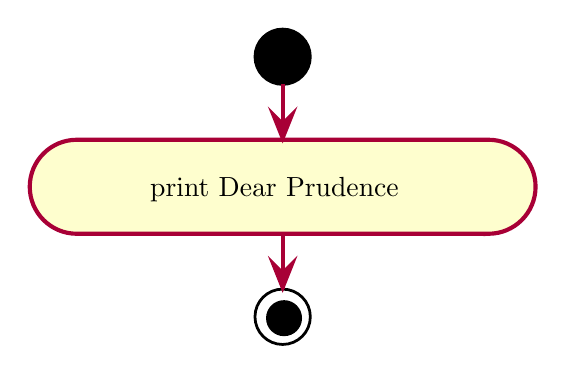
\begin{tikzpicture}[yscale=-1
	,pstyle0/.style={fill=black,line width=1.0pt}
	,pstyle3/.style={color=plantucolor0002,line width=1.5pt}
	,pstyle4/.style={color=plantucolor0002,fill=plantucolor0002,line width=1.0pt}
	]
	\draw[pstyle0] (101.3856pt,20pt) ellipse (10pt and 10pt);
	\draw[color=plantucolor0002,fill=plantucolor0001,line width=1.5pt] (10pt,66.9844pt) arc (180:270:16.9844pt) -- (26.9844pt,50pt) -- (175.7868pt,50pt) arc (270:360:16.9844pt) -- (192.7712pt,66.9844pt) -- (192.7712pt,66.9844pt) arc (0:90:16.9844pt) -- (175.7868pt,83.9688pt) -- (26.9844pt,83.9688pt) arc (90:180:16.9844pt) -- (10pt,66.9844pt) -- cycle;
	\node at (50pt,60pt)[below right,color=black]{print Dear Prudence};
	\draw[color=black,line width=1.0pt] (101.3856pt,113.9688pt) ellipse (10pt and 10pt);
	\draw[pstyle0] (101.8856pt,114.4688pt) ellipse (6pt and 6pt);
	\draw[pstyle3] (101.3856pt,30pt) -- (101.3856pt,50pt);
	\draw[pstyle4] (97.3856pt,40pt) -- (101.3856pt,50pt) -- (105.3856pt,40pt) -- (101.3856pt,44pt) -- cycle;
	\draw[pstyle3] (101.3856pt,83.9688pt) -- (101.3856pt,103.9688pt);
	\draw[pstyle4] (97.3856pt,93.9688pt) -- (101.3856pt,103.9688pt) -- (105.3856pt,93.9688pt) -- (101.3856pt,97.9688pt) -- cycle;
\end{tikzpicture}


\subsection{Quellcode}
\subsubsection{Main.java}
\lstinputlisting[language = Java , frame = trBL , firstnumber = last , escapeinside={(*@}{@*)}]{../chapter_01/src/chapter_01/Main.java}

\subsection{Testdokumentation}
?

\subsection{Benutzungshinweise}
Navigieren Sie in der Kommandozeile zum dem Ordner, wo sich die Java Datei befindet.
Danach führen sie "javac Main.java\dq \space auf. Jetzt können Sie das Programm mit "java main\dq \space
 starten. In der Konsole sollte nun "Dear Prudence\dq \space angeziegt werden.

\subsection{Anwendungsbeispiel}
Nach dem Aufruf von java Main, sollten wir folgendes sehen:
\begin{lstlisting}[frame = trBL , escapeinside={(*@}{@*)}]
[sebastian@laptop bin]$ java Main 
Dear Prudence
[sebastian@laptop bin]$ 
\end{lstlisting}